\newcommand{\codeRef}[2][]{\hyperref[section:#2]{\mintinline{java}!#2#1!}}
\newcommand{\myinput}[3]{\inputminted[frame=single, breaklines=true, linenos=true, firstline=#1, lastline=#2, gobble=#3]{java}{../../src/main/java/userApplication.java}}
\chapter{Η εφαρμογή (\appname{})}
\section{Ρυθμίσεις router}
\begin{figure}[htb]
\centering
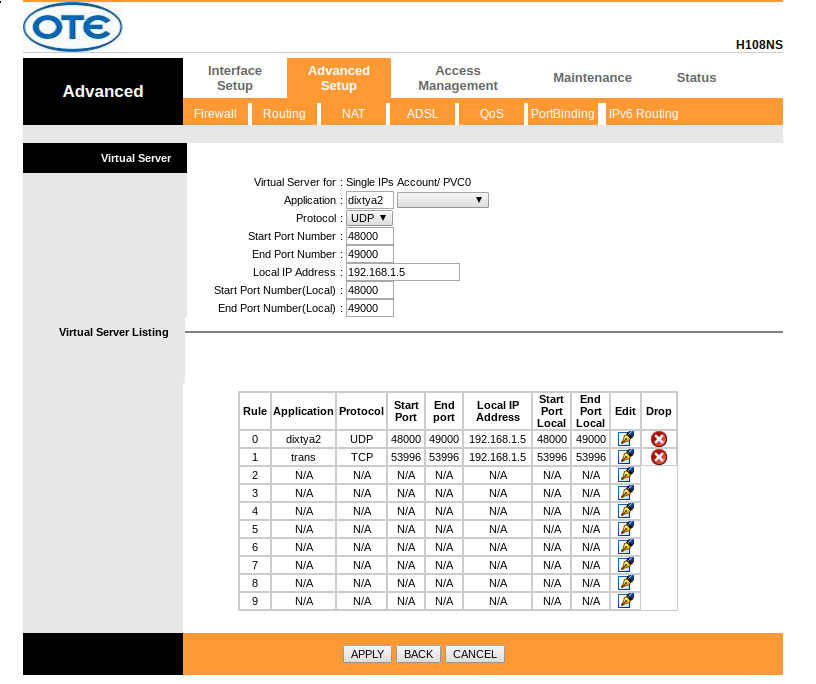
\includegraphics[width=\linewidth]{images/router}
\caption{Ρυθμίσεις router}
\label{fig:router}
\end{figure}
Για την σωστή λειτουργία της εφαρμογής \appname{} χρειάστηκε η αλλαγή ρυθμίσεων του router.
Ακολουθήθηκαν τα εξής βήματα:
\begin{enumerate}
\item Επίσκεψη της σελίδας ρυθμίσεων του router \url{http://192.168.1.1}.
Πρόκειται για μία συσκευή ZTE H108NS, Firmware Version: \texttt{H108NSV1.1.7u\_ZRD\_GR2\_A68}.
\item Εισαγωγή του κωδικού διαχειριστή.
\item Περιήγηση στη σελίδα: \texttt{Advanced Setup > NAT > Virtual Server}.
\item Δημιουργία νέου κανόνα με τις κατάλληλες ρυθμίσεις.
Για τον έλεγχο της ip του μηχανήματος όπου εκτελείται η εφαρμογή εκτελέσαμε:
\begin{code}
\begin{minted}{bash}
$ ifconfig enp2s0
enp2s0: flags=4163<UP,BROADCAST,RUNNING,MULTICAST>  mtu 1500
        inet 192.168.1.5  netmask 255.255.255.0  broadcast 192.168.1.255
        inet6 2a02:587:1808:bb00:5726:d95c:595b:5eae  prefixlen 64  scopeid 0x0<global>
        inet6 fe80::da4c:b00b:629f:ea30  prefixlen 64  scopeid 0x20<link>
        ether 08:60:6e:c7:db:b8  txqueuelen 1000  (Ethernet)
        RX packets 116646  bytes 97594158 (93.0 MiB)
        RX errors 0  dropped 14  overruns 0  frame 0
        TX packets 102421  bytes 56928201 (54.2 MiB)
        TX errors 0  dropped 1 overruns 0  carrier 0  collisions 0
\end{minted}
\caption{Η IP στο τοπικό μηχάνημα}
\end{code}
\begin{code}
\begin{minted}{bash}
$ uname -srmo
Linux 4.4.5-1-ARCH x86_64 GNU/Linux
\end{minted}
\caption{Το λειτουργικό σύστημα του τοπικού μηχανήματος}
\end{code}
Η ρύθμιση φαίνεται στο \imageref{router}.
\end{enumerate}

\section{Script \scriptname{}}\label{section:script}
Για την γρήγορη εξαγωγή των κωδικών από το site \url{http://ithaki.eng.auth.gr/netlab/index.html} γράφτηκε ένα script σε
\href{https://www.python.org/}{python3}
όπου πραγματοποιεί τη σύνδεση (login) με το site με τα σχετικά credentials και εξάγει σε ένα αρχείο τους κωδικούς σε μορφή
\href{https://en.wikipedia.org/wiki/JSON}{json} ώστε να μπορούν εύκολα να διαβαστούν οι τελευταίοι κωδικοί αυτόματα από την εφαρμογή \appname{}.
Χρησιμοποιήθηκαν οι εξωτερικές βιβλιοθήκες:
\begin{itemize}
\item \href{http://docs.python-requests.org/en/master/}{requests} για την πραγματοποίηση της συνεδρίας, και το downloading των σχετικών σελίδων.
\item \href{http://www.crummy.com/software/BeautifulSoup/}{BeautifulSoup} για το parsing των \texttt{.html} αρχείων για την εξαγωγή των κωδικών.
\end{itemize}

Καθώς δεν είναι δυνατό το ανέβασμα επιπλέον αρχείου με το όνομα \scriptname{} ο κώδικας παρατίθεται εδώ:
\begin{code}
\inputminted[frame=single, breaklines=true, linenos=true, python3=true]{python}{../../extract-codes.py}
\caption{Το script για την εξαγωγή των κωδικών}
\end{code}

\section{Script \plotscriptname{}}\label{section:plot-script}
Για την επεξεργασία και απεικόνιση των δεδομένων που προκύπτουν μετά την εκτέλεση της εφαρμογής \appname{} γράφτηκε ένα script επίσης σε \href{https://www.python.org/}{python3}.
Χρησιμοποιήθηκαν οι εξωτερικές βιβλιοθήκες:
\begin{itemize}
\item \href{http://www.numpy.org/}{numpy}
\item \href{https://www.scipy.org/}{scipy}
\item \href{http://matplotlib.org/}{matplotlib}
\end{itemize}

Καθώς δεν είναι δυνατό το ανέβασμα επιπλέον αρχείου με το όνομα \plotscriptname{} ο κώδικας παρατίθεται εδώ:
\begin{code}
\inputminted[frame=single, breaklines=true, linenos=true, python3=true]{python}{../../graphs.py}
\caption{Το script για την απεικόνιση των δεδομένων}
\end{code}

\section{Χρήση βιβλιοθηκών \& imports}
\begin{code}
\myinput{5}{24}{0}
\caption{Imports στο \appname}
\end{code}

Χρησιμοποιήθηκαν οι εξής βιβλιοθήκες:
\begin{itemize}
\item \label{lib:Gson}
\href{https://github.com/google/gson}{\mintinline{java}!com.google.gson.Gson!}:
\begin{displayquote}
Gson is a Java library that can be used to convert Java Objects into their JSON representation. It can also be used to convert a JSON string to an equivalent Java object.
\end{displayquote}
Βιβλιοθήκη της google, για την ανάγνωση και parsing αρχείων τύπου \texttt{JSON}.
Το σχετικό dependency στο maven είναι:
\begin{minted}{xml}
<dependencies>
    <dependency>
        <groupId>com.google.code.gson</groupId>
        <artifactId>gson</artifactId>
        <version>2.6.2</version>
    </dependency>
</dependencies>
\end{minted}
Χρησιμοποιείται αποκλειστικά στη μέθοδο \codeRef[()]{initVariables}.

\item
\href{https://docs.oracle.com/javase/8/docs/api/javax/sound/sampled/package-summary.html}{\mintinline{java}!javax.sound.sampled!}:
\begin{displayquote}
Provides interfaces and classes for capture, processing, and playback of sampled audio data.
\end{displayquote}
Για την αναπαραγωγή ήχου που λαμβάνεται σε μορφή \mintinline{java}!byte[]! (array).
Χρησιμοποιείται στην μέθοδο \codeRef[()]{playMusic}.

\item
\href{https://docs.oracle.com/javase/8/docs/api/java/io/package-summary.html}{\mintinline{java}!java.io.*!}:
\begin{displayquote}
Provides for system input and output through data streams, serialization and the file system.
\end{displayquote}
Χρησιμοποιείται για την διαχείριση αρχείων. Κυρίως για την αποθήκευση των αποτελεσμάτων.

\item
\href{https://docs.oracle.com/javase/8/docs/api/java/net/package-summary.html}{\mintinline{java}!java.net.*!}:
\begin{displayquote}
Provides the classes for implementing networking applications.
\end{displayquote}
Περιλαμβάνει κλάσεις διαχείρισης δικτυακών πόρων.
Παρέχει τις πολύ βασικές κλάσεις για την εφαρμογή μας:
\mintinline{java}!DatagramPacket! και \mintinline{java}!DatagramSocket!.
Χρησιμοποιείται σε όλες τις μεθόδους που έχουν σχέση με τον server της Ιθάκης.

\item
\href{https://docs.oracle.com/javase/8/docs/api/java/nio/package-summary.html}{\mintinline{java}!java.nio!}:
\begin{displayquote}
Defines buffers, which are containers for data, and provides an overview of the other NIO packages.
\end{displayquote}
Χρησιμοποιείται για διάφορες λειτουργικότητες σχετικές με buffers.

\item
\href{https://docs.oracle.com/javase/8/docs/api/java/util/package-summary.html}{\mintinline{java}!java.util!}:
\begin{displayquote}
Contains the collections framework, legacy collection classes, event model, date and time facilities, internationalization, and miscellaneous utility classes (a string tokenizer, a random-number generator, and a bit array).
\end{displayquote}
\sloppy Χρησιμοποιούνται διάφορες βασικές λειτουργίες όπως:
\mintinline{java}!java.util.logging! και \mintinline{java}!java.util.Arrays!.
\end{itemize}

\section{Η κλάση \texttt{userApplication}}
\begin{code}
\begin{minted}{java}
/**
 * Main application for the assignment.
 */
class userApplication {
    private final static Level loggerLevel = Level.ALL;
    private final static Logger logger = Logger.getLogger(userApplication.class.getName());

    static {
        // http://stackoverflow.com/questions/6315699/why-are-the-level-fine-logging-messages-not-showing
        final Handler consoleHandler = new ConsoleHandler();
        consoleHandler.setLevel(loggerLevel);
        logger.setUseParentHandlers(false);
        logger.addHandler(consoleHandler);
        logger.setLevel(loggerLevel);
    }

    public static void main(final String[] args) throws IOException, LineUnavailableException {
        final MainInstance app = new MainInstance();
        app.run(args);
    }

    private static class MainInstance {...}
}
\end{minted}
\caption{Η εξωτερική κλάση \mintinline{java}!userApplication!}
\end{code}
Αποτελεί την εξωτερική κλάση που υλοποιεί την εφαρμογή.
Ρόλος της είναι:
\begin{itemize}
\item Η αρχικοποίηση ενός αντικειμένου \mintinline{java}!Logger logger! που βοηθάει στο debugging και την εκτύπωση μηνυμάτων.
\item Η κλήση της \mintinline{java}!public static void main()! που αρχικοποιεί ένα αντικείμενο της βασικής κλάσης \codeRef[()]{MainInstance}.
\end{itemize}

\section{Η κλάση \texttt{MainInstance}}\label{section:MainInstance}
Αποτελεί την βασική κλάση της εφαρμογής \appname{} και περιλαμβάνει:
σταθερές, μέλη (μεταβλητές) και μεθόδους που σχετίζονται με τη σωστή λειτουργία του κώδικα.

\begin{code}
\myinput{50}{65}{8}
\caption{Σταθερές}
\label{listing:constants}
\end{code}

\begin{code}
\myinput{66}{73}{8}
\caption{Βασικά \mintinline{java}!DatagramSocket! για την επικοινωνία με τον server.}
\end{code}

\begin{code}
\myinput{186}{209}{8}
\caption{Μέλη της κλάσης που κρατάνε τους βασικούς κωδικούς για την επικοινωνία}
\end{code}

\subsection{Constructor \texttt{MainInstance}}
Αρχικοποιεί την κλάση:
\begin{enumerate}
\item Καλεί την \codeRef[()]{initVariables}.
\item Αρχικοποιεί την σύνδεση με τον server μέσω των μεταβλητών \mintinline{java}!client! και \mintinline{java}!server!:
\begin{enumerate}
\item \mintinline{java}!client = new DatagramSocket(clientListeningPort);!.
\item \mintinline{java}!server = new DatagramSocket();!
\item \mintinline{java}!server.connect(address, serverListeningPort);!.
\end{enumerate}
\end{enumerate}

\begin{code}
\myinput{211}{228}{8}
\caption{Constructor της \mintinline{java}!MainInstance!}
\end{code}

\subsection{Το \texttt{interface Decoder}}
Αποτελεί ένα \mintinline{java}!interface! που υλοποιεί τουλάχιστον μία μέθοδο \mintinline{java}!void decode(final byte[] buffer, byte[] decoded, int decodedIndex);!.
Χρησιμοποιείται για την αποκωδικοποίηση ενός \mintinline{java}!byte! array ήχου.
Υπάρχουν 2 αντικείμενα τύπου \mintinline{java}!Decoder! στον κώδικα:
\codeRef[]{dpcmDecoder} και \codeRef[]{aqdpcmDecoder}.
\begin{code}
\myinput{578}{593}{8}
%TODO
\end{code}

\subsubsection{Decoder DPCM: \texttt{dpcmDecoder}}\label{section:dpcmDecoder}
Αντικείμενο τύπου \mintinline{java}!Decoder! που υλοποιεί αποκωδικοποίηση DPCM.
\begin{code}
\myinput{74}{94}{8}
\caption{O \mintinline{java}!Decoder dpcmDecoder!}
\end{code}

Εδώ, η μέθοδος \mintinline{java}!decode()! είναι αρμόδια για την κωδικοποίηση των πακέτων του ήχου σύμφωνα με τις αρχές που διέπουν την απλή διαφορική παλμοκωδική διαμόρφωση DPCM.
Η συγκεκριμένη μέθοδος κανονικοποιεί τη διαφορά δύο διαδοχικών δειγμάτων ήχου που κωδικοποιούνται με 4 bits από την τιμή -8 έως την τιμή +7.
Στη συνέχεια, οι διαδοχικές τιμές διαφορών τοποθετούνται ανά δυο σε ένα byte, αφού προηγουμένως σε κάθε μία τιμή διαφοράς προστεθεί, για λόγους απλοποίησης της εφαρμογής, η τιμή +8, ώστε το κάθε nibble του byte να παριστά θετικό ακέραιο αριθμό μεταξύ των τιμών 0 και 15.
Τα μεταδιδόμενα πακέτα αποτελούνται από 128 bytes ζευγών διαφορών τα οποία αντιστοιχούν σε 256 δείγματα ήχου.
Στο δέκτη, τα δείγματα ήχου 32 τέτοιων πακέτων αναπαραγόμενα με σταθερό ρυθμό 8000 samples/sec αντιστοιχούν περίπου σε 1 δευτερόλεπτο ήχου.
Τελικά, το αποκωδικοποιημένο τμήμα αποθηκεύεται στο array \mintinline{java}!final byte[] decoded!.

\subsubsection{Decoder AQ-DPCM: \texttt{aqdpcmDecoder}}\label{section:aqdpcmDecoder}
Αντικείμενο τύπου \mintinline{java}!Decoder! που υλοποιεί αποκωδικοποίηση AQ-DPCM.
\begin{code}
\myinput{95}{185}{8}
\caption{O \mintinline{java}!Decoder aqdpcmDecoder!}
\end{code}

Εδώ, η μέθοδος \mintinline{java}!decode()! είναι αρμόδια για την προσαρμοζόμενη κωδικοποίηση AQ-DPCM.
Η προσαρμογή γίνεται κάθε 256 δείγματα ήχου προσδιορίζοντας το βήμα ενός βέλτιστου ομοιόμορφου κβαντιστή των 4 bits
με βάση την υπόθεση κανονικής κατανομής των τιμών των διαφορών (Gaussian error distribution).
Οι τιμές των διαφορών αυτών υπολογίζονται, κωδικοποιούνται και τοποθετούνται σε πακέτα των 128 bytes.
Η μέση τιμή καθώς και το βήμα του κβαντιστή των 256 δειγμάτων ήχου κωδικοποιούνται, ως προσαρμοζόμενες παράμετροι κωδικοποίησης,
γραμμικά με ακρίβεια 16 bits και οι τιμές τους τοποθετούνται σε 4 bytes, τα οποία προηγούνται του πακέτου των 128 bytes των διαφορών.
Το σύνολο αποστέλλεται ως ένα ενιαίο πακέτο UDP μήκους 132 bytes.
Η μέθοδος \mintinline{java}!decode()! λαμβάνει τις τιμές αυτές μέσω της μεθόδου \mintinline{java}!getInt()! όπου χρησιμοποιεί ένα αντικείμενο τύπου \mintinline{java}!ByteBuffer! και μετατρέπει 2 byte σε ακέραιο θεωρώντας little endian format (το λιγότερο σημαντικό byte προηγείται του πλέον σημαντικού byte).

\subsection{Η μέθοδος \texttt{initVariables}}\label{section:initVariables}
Αρχικοποιεί τους κωδικούς για την σύνδεση με τον server.
Απαιτεί την ύπαρξη του αρχείου \texttt{codes.json} το οποίο δημιουργείται μέσω της εκτέλεσης του \scriptname{} (ή και χειροκίνητα).
Χρησιμοποιεί την βιβλιοθήκη \hyperref[lib:Gson]{Gson}.
\begin{code}
\myinput{550}{576}{8}
\caption{Η μέθοδος \mintinline{java}!initVariables()!}
\end{code}

\subsection{Η μέθοδος \texttt{simpleSend}}\label{section:simpleSend}
Αποτελεί μέθοδο που στέλνει ένα απλό μήνυμα \mintinline{java}!String message! στον server της Ιθάκης.
Δημιουργείται ένας \mintinline{java}!byte[] buffer! και ένα νέο \mintinline{java}!DatagramPacket packet! που αποστέλλεται μέσω του \mintinline{java}!DatagramSocket server!.
\begin{code}
\myinput{291}{302}{8}
\caption{Η μέθοδος αποστολής απλού μηνύματος \mintinline{java}!simpleSend()!}
\end{code}

\subsection{Η μέθοδος \texttt{testThroughput}}
Αποτελεί την μέθοδο που αναλαμβάνει την αποστολή και χρονομέτρηση για τουλάχιστον 4 λεπτά πακέτων τύπου \texttt{ECHO} στον server.
Η χρονομέτρηση της απόκρισης γίνεται μέσω της \mintinline{java}!System.currentTimeMillis()!.
Το αποτέλεσμα αποθηκεύεται σε ένα αρχείο με όνομα \mintinline{java}!code + ".txt"! ώστε να μπορεί να διαβαστεί από το script που δημιουργεί τις γραφικές παραστάσεις.
Η πληροφορία του χρόνου απόκρισης αποθηκεύεται σε μια γραμμή για κάθε πακέτο.
\begin{code}
\myinput{304}{345}{8}
\caption{Η μέθοδος για την χρονομέτρηση της απόκρισης, \mintinline{java}!testThroughput()!}
\end{code}

\subsection{Οι συναρτήσεις \texttt{downloadSound}}\label{section:downloadSound}
\subsubsection{Βασική μέθοδος \texttt{downloadSound}}
Περιλαμβάνει τον βασικό κώδικα που αναλαμβάνει την λήψη bytes ήχου.
\begin{code}
\myinput{401}{460}{8}
\caption{Κυρίως κώδικας για λήψη ήχου στη \mintinline{java}!downloadSound()!}
\end{code}

Η λειτουργία της δομείται ως εξής:
\begin{enumerate}
    \item Κατασκευάζεται ανάλογα με τα ορίσματα η εντολή που θα σταλεί στον server και μετά στέλνεται μέσω της \codeRef[()]{simpleSend}:
    \begin{enumerate}
        \item Η εντολή αρχίζει με τον κωδικό \mintinline{java}!soundRequestCode! μαζί με το νούμερο του τραγουδιού σε μορφή \mintinline{java}!"LXX"!
        (βλ. \hyperref[section:downloadSound-overload]{Overload μεθόδου \mintinline{java}!downloadSound()!}).

        \item Αν χρησιμοποιείται αποκωδικοποίηση AQ (\mintinline{java}!boolean useAQ!) προστίθενται οι χαρακτήρες \mintinline{java}!"AQ"!.

        \item Αν θέλουμε τυχαίο ήχο (\mintinline{java}!boolean randomTrack!) προστίθεται ο χαρακτήρας \mintinline{java}!"T"! αλλιώς \mintinline{java}!"F"!.

        \item Προστίθεται ο αριθμός \mintinline{java}!totalPackages! των πακέτων ήχου που αποστέλλονται από τον server σε μορφή \mintinline{java}!"XXX"!.
    \end{enumerate}
    \begin{minted}{java}
    final String command = soundRequestCode + trackCode + (useAQ ? "AQ" : "") + (randomTrack ? "T" : "F") + String.format("%03d", totalPackages);
    simpleSend(command);
    \end{minted}

    \item Σε περίπτωση χρήσης AQ επιλέγεται ο \mintinline{java}!aqdpcmDecoder! αλλιώς ο \mintinline{java}!dpcmDecoder!.
    \begin{minted}{java}
    Decoder decoder = useAQ ? aqdpcmDecoder : dpcmDecoder;
    \end{minted}

    \item Αρχικοποιούνται: ένας buffer, ένα \mintinline{java}!DatagramPacket packet! και ένας πίνακας byte όπου θα αποθηκευτεί το αποκωδικοποιημένο αποτέλεσμα \mintinline{java}!byte[] decoded! με κατάλληλα μεγέθη.
    \begin{minted}{java}
    // Received packets for DPCM are 128 bytes long and 132 bytes long for AQ-DPCM.
    final int audioStepPerBufferByte = (useAQ ? 4 : 2);
    final byte[] buffer = new byte[AUDIO_PACKAGE_LENGTH + (useAQ ? 4 : 0)];
    final byte[] decoded = new byte[audioStepPerBufferByte * AUDIO_PACKAGE_LENGTH * totalPackages];
    final DatagramPacket packet = new DatagramPacket(buffer, buffer.length);
    \end{minted}

    \item Λαμβάνεται ο αριθμός των πακέτων που προσδιορίστηκε μέσω του \mintinline{java}!DatagramSocket client!.
    Για κάθε πακέτο καλείται Η μέθοδος \mintinline{java}!decode()!.
    \begin{minted}{java}
    for (int packageId = 0; packageId < totalPackages; packageId++) {
        client.receive(packet);
        decoder.decode(buffer, decoded, audioStepPerBufferByte * AUDIO_PACKAGE_LENGTH * packageId);
    }
    \end{minted}

    \item Επιστρέφεται το αποκωδικοποιημένο κομμάτι ήχου (\mintinline{java}!byte[] decoded!).
\end{enumerate}

\subsubsection{Overload μεθόδου \texttt{downloadSound}}\label{section:downloadSound-overload}
Λαμβάνει όρισμα \mintinline{java}!int trackId! και το μετατρέπει σε κατάλληλο \mintinline{java}!String! που μπορεί να το δεχτεί ο server της Ιθάκης.
\begin{code}
\myinput{379}{399}{8}
\caption{Μέθοδος \mintinline{java}!downloadSound()! με όρισμα \mintinline{java}!int trackId!}
\end{code}

\subsubsection{Η \texttt{downloadRandomSound}}
Καλεί την \mintinline{java}!downloadSound()! με κατάλληλα ορίσματα ώστε να ληφθεί ήχος μέσω της εικονικής γεννήτριας συχνοτήτων του server της Ιθάκης.
\begin{code}
\myinput{364}{377}{8}
\caption{Μέθοδος \mintinline{java}!downloadRandomSound()!}
\end{code}

\subsection{Η μέθοδος \texttt{playMusic}}\label{section:playMusic}
Η συγκεκριμένη μέθοδος είναι υπεύθυνη για την αναπαραγωγή της μουσικής που έχει ληφθεί από τον server.
Δέχεται σαν όρισμα τη μεταβλητή \mintinline{java}!byte[] audio! που περιέχει την πληροφορία του αποκωδικοποιημένου ήχου.
Επίσης, δέχεται όρισμα \mintinline{java}!int Q! τον αριθμό bits του κβαντιστή που χρησιμοποιείται κατά την αναπαραγωγή του ήχου.
\begin{code}
\myinput{347}{362}{8}
\caption{Η μέθοδος αναπαραγωγής ήχου \mintinline{java}!playMusic()!}
\end{code}

\subsection{Η μέθοδος \texttt{downloadImage}}
Αποτελεί την μέθοδο που αναλαμβάνει την επικοινωνία με τον server για την λήψη εικόνας.
\begin{code}
\myinput{480}{540}{8}
\caption{Η μέθοδος για την λήψη εικόνας \mintinline{java}!downloadImage()!}
\end{code}

Η λειτουργία της δομείται ως εξής:
\begin{enumerate}
    \item Κατασκευάζεται ανάλογα με τα ορίσματα η εντολή που θα σταλεί στον server και μετά στέλνεται μέσω της \codeRef[()]{simpleSend}:
    \begin{enumerate}
        \item Η εντολή αρχίζει με τον κωδικό \mintinline{java}!imageRequestCode!.

        \item Αν χρησιμοποιείται η λειτουργία "flow" (απλός μηχανισμός ελέγχου ροής πακέτων κατά τη λήψη της εικόνας, \mintinline{java}!boolean useFlow!) προστίθενται οι χαρακτήρες \mintinline{java}!"FLOW=ON"!.

        \item Προστίθενται οι χαρακτήρες \mintinline{java}!"UDP="! και ο αριθμός \mintinline{java}!maxLength!
        που δηλώνει σε bytes το μήκος του τμήματος info των πακέτων UDP που χρησιμοποιεί ο server για την αποστολή της εικόνας.

        \item Προστίθενται οι χαρακτήρες \mintinline{java}!"CAM="! και ο κωδικός της κάμερας που θα χρησιμοποιηθεί (\mintinline{java}!"FIX"! ή \mintinline{java}!"PTZ"!).
    \end{enumerate}
    \begin{minted}{java}
    final String imageCommand = imageRequestCode + (useFlow ? "FLOW=ON" : "") + "UDP=" + maxLength + "CAM=" + camera;
    simpleSend(imageCommand);
    \end{minted}

    \item Σε ένα βρόχο επανάληψης λαμβάνονται τα πακέτα UDP με την πληροφορία της εικόνας. Η διαδικασία σταματάει άν γίνει timeout ή αν ληφθεί πακέτο μικρότερου μήκους.
    \begin{minted}{java}
    final int packetLength = imagePacket.getLength();
    logger.finest(filename + ": Received image packet of length:" + packetLength + ".");
    stream.write(imageBuffer, 0, packetLength);
    if (packetLength < maxLength) {
        break;
    }
    \end{minted}

    \item Σε κάθε επανάληψη, μετά την λήψη, αν είναι ενεργοποιημένη η λειτουργία "FLOW", στέλνεται η ένδειξη \mintinline{java}!"NEXT"! στον server.
    \begin{minted}{java}
    if (useFlow) {
        simpleSend("NEXT");
    }
    \end{minted}

    \item Το αποτέλεσμα αποθηκεύεται σε ένα αρχείο με όνομα \mintinline{java}!filename! (όρισμα της μεθόδου).
\end{enumerate}
